\section{Lifted Inference using Embeddings}

We generate a low-dimensional neural embedding for the MLN objects using a model we call Obj2Vec, where approximately symmetric objects lie close to each other in the embedding. 
%To achieve this, we encode objects in the MLN that share a ground formula as sentences, and run Word2vec to this encoding to learn the symmetry between objects, using which we can reduce the number of objects in the MLN.
%. Specifically, the general idea behind our approach is that symmetric objects share similar contexts in the MLN formulas. Therefore, learning a low-dimensional embedding  for the objects based on their context will
%Specifically,  symmetric objects in the MLN are likely to be close to each other in the embedded vector-space. To achieve this, we encode objects that share a ground formula in the MLN as sentences such that symmetrical objects yield similar sentences in our model. We next run Word2vec on the encoded objects to generate their embedding in a lower dimension. 
To formalize our approach, we assume that our MLN has $n$ domains $\Delta_1$, $\Delta_2$ $\ldots$ $\Delta_n$.  Let $\mathcal{D}$ be the evidence database presented to the MLN,  $f_1$ $\ldots$ $f_k$ be the MLN formulas, and ${\tt R}_1$ $\ldots$ ${\tt R}_p$ be the predicates. Our task is to embed the set of domains $\Delta_1$, $\Delta_2$ $\ldots$ $\Delta_n$ into a lower-dimensional space, and use similarity of the objects in the embedded space to reduce the size of the domains, and create a new domain-set $\hat{\Delta}_1$, $\hat{\Delta}_2$ $\ldots$ $\hat{\Delta}_n$, where $|\hat{\Delta}_i|$ $\leq$ $|{\Delta}_i|$.
 
 \subsection{Obj2Vec}
\begin{figure} 
\centering
 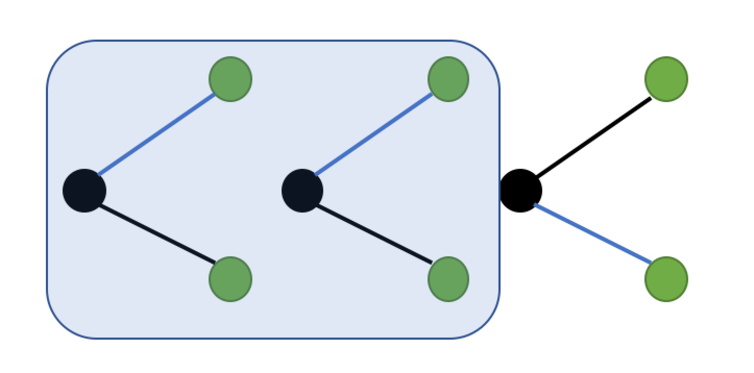
\includegraphics[scale=0.55]{ex1.pdf}
 \caption{\label{fig:ex1}Markov network for ${\tt R}(x)$ $\wedge$ ${\tt S}(x,y)$. The green nodes correspond to ${\tt S}$ and black nodes to ${\tt R}$. The blue line indicates that the grounding corresponding to that potential is satisfied by the evidence given by ${\tt R}(X_1)$, ${\tt R}(X_2)$, ${\tt R}(X_3)$, ${\tt S}(X_1,Y_1)$, ${\tt S}(X_2,Y_1)$, ${\tt S}(X_3,Y_2)$. The groundings corresponding to $X_1$ and $X_2$ are symmetric.}
 \end{figure}
 
 
Consider a simple formula ${\tt R}(x)$ $\wedge$ ${\tt S}(x,y)$. Let $\Delta_x$ $=$ $\{X_1,X_2,X_3\}$ and $\Delta_y$ $=$ $\{Y_1,Y_2\}$. Let the evidence database be ${\tt R}(X_1)$, ${\tt R}(X_2)$, ${\tt R}(X_3)$, ${\tt S}(X_1,Y_1)$, ${\tt S}(X_2,Y_1)$, ${\tt S}(X_3,Y_2)$. The objects $X_1$ and $X_2$ are symmetrical since they can be exchanged in the groundings in which they appear without changing the MLN as shown in Fig.~\ref{fig:ex1}. Specifically, they appear  along with similar objects (in this case $Y_1$) in ground formulas of the MLN. Using this, we can define the context as follows.

 \begin{definition}
 Let $\bar{f}$ be a ground formula satisfied by evidence $\mathcal{D}$. We define the context of any object in $\bar{f}$  as the set of other objects in $\bar{f}$ .
 \end{definition}

Our idea is to detect symmetries based on the above-defined context. For this, consider the following encoding for the MLN objects, where for every satisfied ground formula, we list the objects that appear in the context of each other. Therefore, for our previous example, the encoding is, $X_1Y_1;X_2Y_1;X_3Y_2$. Analogous to the input to skip-gram models, we can think of each ground formula as being encoded as a ``sentence'' in a document, where the sentences are shown to be separated by a ``;'. The pair $X_1Y_1$ encodes that $X_1$ has a context $Y_1$ in some grounding of the MLN formula. Notice that $X_2$ also has a context $Y_1$.

%Clearly, the objects $X_1$ and $X_2$ are symmetrical since they  



%Clearly, the ground formulas ${\tt R}(X_1)$ $\wedge$ ${\tt S}(X_1,Y_1)$ and ${\tt R}(X_2)$ $\wedge$ ${\tt S}(X_2,Y_1)$ are symmetrical due to the evidence presented. context in which these objects appear. Specifically, both $X_1$ and $X_2$ appear along with $Y_1$ 


%Consider the following encoding of the MLN, $X_1Y_1;X_2Y_1;X_3Y_2$, where sentences are shown to be separated by a ``;''. The pair $X_1Y_1$ encodes that $X_1$ has a dependency with $Y_1$ in some grounding of the MLN formula. Notice that $X_2$ also has a dependency with $Y_1$. Thus, $X_1$ and $X_2$ are symmetrical to each other. 

Now let us consider a neural network architecture that will work on our input encoding. Specifically, the network architecture we use is the same as is used in skip-gram models such as Word2Vec. For Word2vec, the context is defined by a small fixed-size window of words in a document, while for Obj2vec, the context is the objects in a ground formula that is satisfied by the evidence. Therefore, just as in skip-gram models, from each of our encoded sentences $X_1Y_1$, $X_2Y_1$ and $X_3Y_2$, we generate input/output pairs, where we predict an object given another object from its context. That is, given $X_1$ or $X_2$ at the input layer, we predict $Y_1$ at the output layer, and given $X_3$ as input we predict $Y_2$ as the output layer. This means that the hidden layer in the model will derive features such that $X_1$ and $X_2$ will make common predictions at the output layer. Therefore, the hidden layer representation for both $X_1$ and $X_2$ should be similar indicating symmetry of $X_1$ and $X_2$. As the context surrounding both $X_1$ and $X_2$ becomes more and more similar, the embedding for $X_1$ and $X_2$ grows closer to each other.  At the same time, since $X_3$ has a different context, it needs to predict $Y_2$ at the output layer, and therefore, the hidden layer encoding for $X_3$ will be different from that of $X_1$ and $X_2$. 
%Now, say $X_3$ relates with common objects as $X_1$ and $X_2$ on other groundings on the MLN, the hidden layer embedding for $X_3$ will grow closer to that of $X_1$ and $X_2$ indicating symmetry between the objects.

\begin{figure} 
\centering
 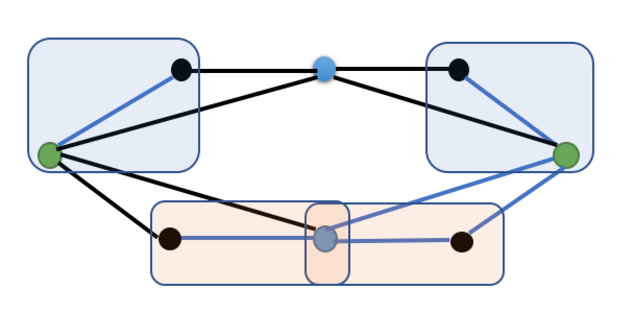
\includegraphics[scale=0.65]{ex2.pdf}
 \caption{\label{fig:ex2}Markov network for ${\tt R}(x)$ $\wedge$ ${\tt S}(x,y)$ $\wedge$ ${\tt T}(y)$. The green nodes correspond to ${\tt R}$, black nodes to ${\tt S}$ and blue nodes to ${\tt T}$. The blue line indicates that the partial grounding corresponding to that potential is satisfied by the evidence given by ${\tt R}(X_1)$, ${\tt S}(X_1,Y_1)$, ${\tt R}(X_2)$, ${\tt S}(X_2,Y_1)$, ${\tt S}(X_2,Y_2)$, ${\tt T}(Y_2)$. Symmetries are shown as shaded regions.}
 \end{figure}

To generalize the above, let $D$ be the ``document'' we generate from $\Delta_1$, $\Delta_2$ $\ldots$ $\Delta_n$  by encoding the object contexts as sentences. Let $\bar{f}_i^j$ be the $j$-th grounding of the $i$-th formula. We now have two cases, $\bar{f}_i^j$ is satisfied by the evidence $\mathcal{D}$, or $\bar{f}_i^j$  is unsatisfied by $\mathcal{D}$. If $\bar{f}_i^j$ is satisfied by $\mathcal{D}$, we encode the the ground objects in $\bar{f}_i^j$ as a sentence in  $D$, indicating the context of the objects in $\bar{f}_i^j$. If $\bar{f}_i^j$ is not satisfied by $\mathcal{D}$, then we do not encode it in $D$. This is because, the context is not supported by the observed evidence. 

\noindent{\bf Partial Symmetries}. One of the consequences of encoding context only based on formulas satisfied by $\mathcal{D}$ is that we lose symmetries of partially satisfied formulas. For example, consider the following MLN, ${\tt R}(x)$ $\wedge$ ${\tt S}(x,y)$ $\wedge$ ${\tt T}(y)$. Let our evidence be ${\tt R}(X_1)$, ${\tt S}(X_1,Y_1)$, ${\tt R}(X_2)$, ${\tt S}(X_2,Y_1)$, ${\tt S}(X_2,Y_2)$, ${\tt T}(Y_2)$. The Markov network corresponding to the MLN is shown in Fig.~\ref{fig:ex2}. As shown here, there are some partial symmetries, even though the ground formulas are not satisfied by the evidence. Using our aforementioned encoding, since only one ground formula is satisfied by $\mathcal{D}$, our encoding produced is $X_2Y_1$. Therefore we cannot detect the symmetries that exist between $X_1$ and $X_2$ w.r.t the predicates ${\tt R}$ and ${\tt S}$, and the symmetries between $Y_1$ and $Y_2$ w.r.t predicates ${\tt S}$ and ${\tt T}$. Therefore, we modify our approach slightly to make it more fine-grained by encoding the context for objects for every pair of predicates in the MLN. The idea is that, for a pair of predicates, if the evidence shows that objects share a context, then it is possible that there are some symmetries between those objects. That is, let ${\tt R}_i$ and ${\tt R}_j$ be a predicate pair. For every formula $f_i$ where both ${\tt R}_i$ and ${\tt R}_j$ occur, we eliminate all predicates from $f_i$ other than ${\tt R}_i$ and ${\tt R}_j$, along with their preceding logical connectives. For example, ${\tt R}_i(x,y)$ $\wedge$ ${\tt R}_k(y,z)$ $\Rightarrow$ ${\tt R}_j(z,x)$ reduces to ${\tt R}_i(x,y)$ $\Rightarrow$ ${\tt R}_j(z,x)$. For each grounding of the modified formula, if the evidence $\mathcal{D}$ satisfies the formula, we encode the objects in the grounding as a sentence in our document $D$. Note that dependencies on self-joined predicates can be naturally handled using this approach by pairing ${\tt R}_i$ with itself.

\begin{figure}
\subfigure[]{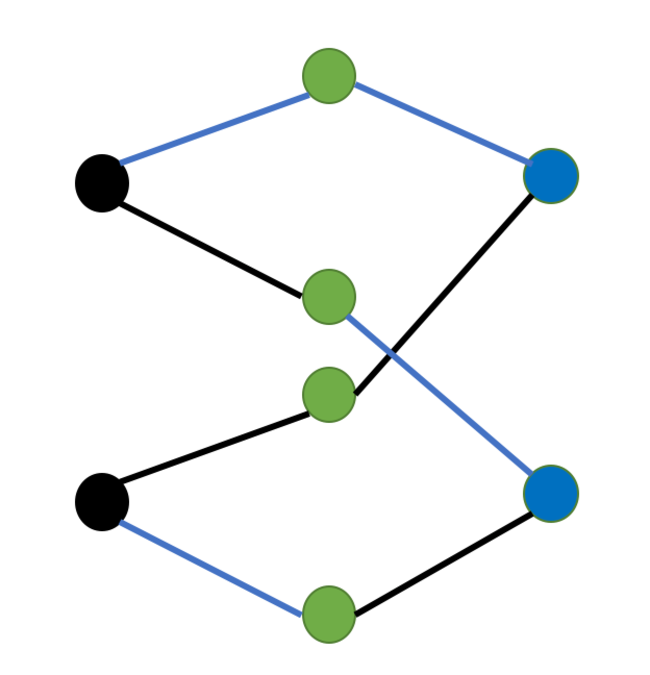
\includegraphics[scale=0.35]{ex3a.pdf}}
\subfigure[]{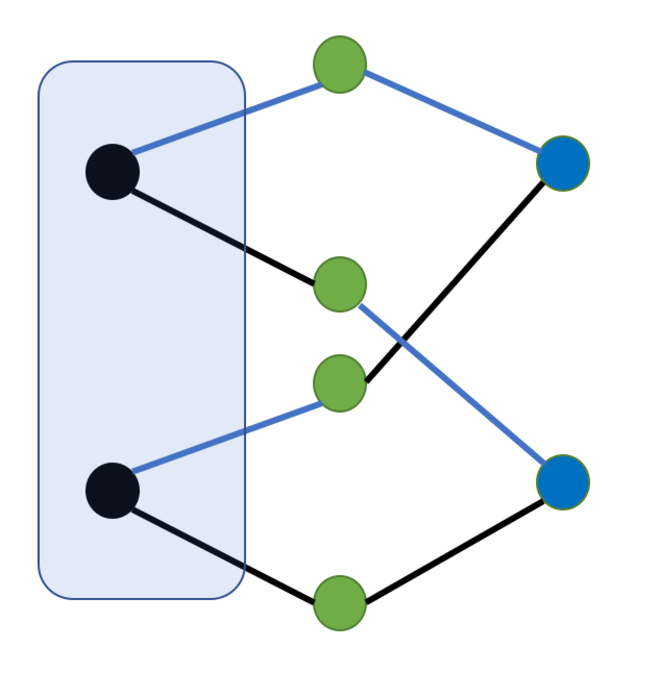
\includegraphics[scale=0.35]{ex3b.pdf}}
\caption{\label{fig:ex3}Markov network for ${\tt R}(x)$ $\wedge$ ${\tt S}(x,y)$; ${\tt S}(x,y)$ $\wedge$ ${\tt T}(y)$. The black nodes correspond to ${\tt R}$, green nodes to ${\tt S}$ and blue nodes to ${\tt T}$. The blue line indicates that the grounding corresponding to that potential is satisfied by the evidence. (a) shows the original Markov network. Due to the symmetries when we we consider the pair ${\tt S}$ and ${\tt T}$, we can interchange some of the links between ${\tt R}$ and ${\tt S}$, and detect symmetries on objects corresponding to $x$ as shown in (b).}
\end{figure}
\noindent{\bf Joint Symmetries}. One of the advantages of our approach is that symmetries on one object can affect symmetries on another object. For example, consider the formulas ${\tt R}(x)$ $\wedge$ ${\tt S}(x,y)$; ${\tt S}(x,y)$ $\wedge$ ${\tt T}(y)$. Suppose $Y_1$ and $Y_2$ appear in the same context w.r.t  ${\tt S}$ and ${\tt T}$ in several cases. The embedding for $Y_1$ and $Y_2$ will become similar in the hidden-layer of Obj2vec. Now suppose $X_1$ has a context $Y_1$, and $X_2$ has a context $Y_2$, then, due to the similarity of $Y_1$ and $Y_2$, even though $X_1$ and $X_2$ have differing contexts, the embedding for $X_1$ grows closer to $X_2$. This is illustrated in Fig.~\ref{fig:ex3}. Here (a) shows the Markov network for our example MLN given evidence ${\tt R}(X_1)$, ${\tt S}(X_1,Y_1)$, ${\tt R}(X_2)$, ${\tt S}(X_2,Y_2)$, ${\tt S}(X_1,Y_1)$, ${\tt S}(X_1,Y_2)$, ${\tt T}(Y_1)$, ${\tt T}(Y_2)$. Due to the symmetries on $Y_1$ and $Y_2$ (they both have same context $X_1$), we can exchange the color of the links between ${\tt R}(X_2)$, ${\tt S}(X_2,Y_1)$ and ${\tt R}(X_2)$, ${\tt S}(X_2,Y_2)$. This changes the the Markov network as shown in (b), and we can notice symmetries between $X_1$ and $X_2$. Thus, in general, we can propagate symmetries across domains, which would help us uncover more complex symmetries in the MLN that are hard to detect when independently clustering the domains.
%Specifically, let ${\tt P}$ and  ${\tt Q}$ be two predicates in our MLN. For every formula, we compute the dependencies between ${\tt P}$ and  ${\tt Q}$, and encode it in $D$. That is, for a formula $f_i$, we eliminate all predicates other than ${\tt P}$ and  ${\tt Q}$, along with the logical connective succeeding each of the eliminated predicates. For each grounding of the modified formula, if the evidence $\mathcal{D}$ satisfies the formula, we include the objects for which the formula is satisfied as a sentence in our document $D$. Note that dependencies on self-joined predicates can be naturally handled using this approach by pairing predicates with themselves.







%Let the evidence database be ${\tt R}(X_1,Y_1)$, ${\tt R}(X_1,Y_1)$, ${\tt R}(X_1,Y_1)$, ${\tt R}(X_1,Y_1)$, ${\tt S}(X_1,Y_1)$, ${\tt S}(X_2,Y_1)$, ${\tt S}(X_3,Y_2)$. 

%To do this, we encode the domain based on their relational dependencies with other domain objects in the MLN. 
%On the other hand, if our evidence database shows that, $X_1$ and $X_2$ 

%We now describe our approach to create a neural embedding of the MLN's domain. We would want objects that appear together with similar objects in MLN formulas to be close to each other in the embedded space. 

%For this, we encode groundings of MLN formulas as sentences in a document. 


%However, since considering all possible ground formulas is computationally expensive, we consider the interaction between subsets of predicates and compute our sentences from these subsets. We then use Word2vec to generate embeddings of objects, and reduce the objects based on the distance between object vectors in the embedded vector-space.

%\subsection{Encoding}

%Let ${\tt A}_1$ $\ldots$ ${\tt A}_m$ be the predicates in our MLN, let $\Delta_1$, $\Delta_2$ $\ldots$ $\Delta_n$ be the domains of the MLN computed from the evidence database $\mathcal{D}$. Let ${\bf X}$ be a possible subset of predicates of size $k$. For every formula $f$ in the MLN where ${\bf X}$ occurs, we compute the possible groundings for ${\bf X}$ from $f$, and encode them as sentences in our document. 
\eat{
\begin{example}
Let $w$ ${\tt R}(x)$ $\wedge$ ${\tt S}(x,y)$ be a single-formula MLN. We will 
\end{example}
}

%We consider all possible subset of predicates of size $k$, and encode the objects in $\Delta_1$, $\Delta_2$ $\ldots$ $\Delta_n$ as follows